\documentclass[a4paper,12pt]{article}

\usepackage[utf8]{inputenc}
\usepackage[T1]{fontenc}
\usepackage[a4paper,total={150mm,240mm}]{geometry}
\usepackage{amsmath}
\usepackage{amsfonts}
\usepackage{amsthm}
\usepackage{amscd}
\usepackage{grffile}
\usepackage{tikz} 
\usepackage{eurosym} 
\usepackage{graphicx}
\usepackage{color}
\usepackage{listings}
\lstset{language=C++, basicstyle=\ttfamily, 
  keywordstyle=\color{black}\bfseries, tabsize=4, stringstyle=\ttfamily,
  commentstyle=\itshape, extendedchars=true, escapeinside={/*@}{@*/}}
\usepackage{paralist}
\usepackage{curves}
\usepackage{calc}
\usepackage{picinpar}
\usepackage{enumerate}
\usepackage{algpseudocode}
\usepackage{bm}
\usepackage{multibib}
\usepackage{hyperref}
\usepackage{textcase}
\usepackage{nicefrac}

\definecolor{listingbg}{gray}{0.95}

\title{DUNE PDELab Tutorial 01 \\ 
Conforming Finite Element Method for a Nonlinear Poisson Equation}
\author{DUNE/PDELab Team}
\date{\today}

\begin{document}

\maketitle
\tableofcontents
\clearpage

\section{Introduction}

In this tutorial we extend tutorial 00 in the following ways:
\begin{enumerate}[1)]
\item Solve a nonlinear stationary partial differential equation (PDE).
\item Use conforming finite element spaces of arbitrary order.
\item Use different types of (conforming) meshes (simplicial, cubed and mixed).
\item Use multiple types of boundary conditions.
\end{enumerate}
Combined with the fact that the implementation works in any dimension
(note: it is not claimed to be efficient in high dimension $d>3$) this comprises
already a relatively large space of different methods, so the example illustrates
the flexibility of PDELab. Moreover, the 
finite element method developed in this tutorial will serve as a 
building block for instationary problems, adaptive mesh refinement and
parallel solution in subsequent tutorials.

\subsection*{Depends On} 

This tutorial depends on tutorial 00 which discusses piecewise linear elements on simplicial
elements. It is assumed that you have worked through tutorial 00 before.

\section{Problem Formulation}

Here we consider the following nonlinear Poisson equation with
Dirichlet and Neumann boundary conditions:
\begin{subequations} \label{eq:ProblemStrong}
\begin{align}
-\Delta u + q(u) &= f &&\text{in $\Omega$},\\
u &= g &&\text{on $\Gamma_D\subseteq\partial\Omega$},\\
-\nabla u\cdot \nu &= j &&\text{on $\Gamma_N=\partial\Omega\setminus\Gamma_D$}.
\end{align}
\end{subequations}
$\Omega\subset\mathbb{R}^d$ is a domain, $q:\mathbb{R}\to\mathbb{R}$ is a given, possibly
nonlinear function and $f: \Omega\to\mathbb{R}$ is the source term and
$\nu$ denotes the unit outer normal to the domain.

The weak formulation of this problem is derived by multiplication with an appropriate
test function and integrating by parts. This results in the abstract problem:
\begin{equation}
\text{Find $u\in U$ s.t.:} \quad r^{\text{NLP}}(u,v)=0 \quad \forall v\in V,
\label{Eq:BasicBuildingBlock}
\end{equation}
with the continuous residual form
\begin{equation*}
r^{\text{NLP}}(u,v) = \int_\Omega \nabla u \cdot \nabla v + (q(u)-f)v\,dx + \int_{\Gamma_N} jv\,ds
\label{eq:ResidualForm}
\end{equation*}
and the function spaces 
$U= \{v\in H^1(\Omega) \,:\, \text{``$v=g$'' on $\Gamma_D$}\}$
and $V= \{v\in H^1(\Omega) \,:\, \text{``$v=0$'' on $\Gamma_D$}\}$. 
We assume that $q$ is such that this problem has a unique solution.

\section{Finite Element Method}

The finite element method \cite{WHElliptisch,Brenner,Eriksson,Ciarlet,Braess,Ern,Elman2005} 
replaces the function spaces $U$ and $V$ by
finite dimensional approximations defined on a finite element mesh.
Before describing exactly how these spaces are constructed let us
explore the consequences of this.

\subsection{Algebraic Problem}

Any finite-dimensional function space is spanned by a basis. So, assume that
\begin{equation*}
U_h=\text{span}\{\phi_1,\ldots,\phi_n\}, \quad V_h=\text{span}\{\psi_1,\ldots,\psi_m\}
\end{equation*}
are corresponding sets of basis functions for $U_h$ and $V_h$.
Expanding the solution $u_h=\sum_{j=1}^n (z)_j\phi_j$ in the basis and
hereby introducing the coefficient vector $z\in\mathbb{R}^n$ we can
reformulate the problem as
\begin{align*}
\text{Find $u_h\in U_h$ s.t.:} && r(u_h,v)&=0 && \forall v\in V_h\\
\Leftrightarrow{} && r\left(\sum_{j=1}^n (z)_j\phi_j,\psi_i\right) &= 0 &&\forall i=1,\ldots,m\\
\Leftrightarrow{} && R(z) = 0,
\end{align*}
where $R: \mathbb{R}^n \to \mathbb{R}^m$ given by 
$R_i(z) = r_h\left(\sum_{j=1}^n (z)_j\phi_j,\psi_i\right)$ is a nonlinear, vector-valued function.

The solution of the nonlinear algebraic equation $R(z)=0$ is typically computed
in an iterative fashion using e.g. a fixed-point iteration of the form
\begin{equation}
z^{(k+1)} = z^{(k)} - \lambda^{k} W(z^{(k)}) R(z^{(k)}) .
\end{equation}
Here $\lambda^{k}$ is a damping factor
and $W(z^{(k)})$ is a preconditioner matrix, e.g. in Newton's method (see e.g. \cite{Braess}) one
has 
\begin{equation*}
W(z^{(k)}) = (J(z^{(k)}))^{-1} \quad \text{where $(J(z^{(k)}))_{i,j} = \frac{\partial R_i}{\partial z_j}
(z^{(k)})$}
\end{equation*}
(we now assumed that $n=m$ and that the Jacobian $J(z^{(k)})$ is invertible).
Newton's method requires the solution of the linear system $J(z^{(k)}) w = R(z^{(k)})$ in each
step which could be done using either direct or iterative methods.
The implementation of  Newton's method requires the following
algorithmic building blocks:
\begin{enumerate}[i)]
\item residual evaluation $R(z)$,
\item Jacobian evaluation $J(z)$ (or an approximation of it),
\item matrix-free Jacobian application $J(z) w$ (or an approximation).
\end{enumerate}
Only one of the methods ii) and iii) is required depending on the chosen
solution procedure.

\subsubsection*{A Note on Matrix-free Evaluation}

The matrix-free multiplication of the Jacobian $J(z)$ with a vector $w$ is with
the definitions above:
\begin{equation*}
(J(z) w)_i = \sum_{j=1}^n (J(z))_{i,j} (w)_j = \sum_{j=1}^n 
\frac{\partial}{\partial z_j} r_h\left(\sum_{l=1}^n (z)_l  \phi_l,\psi_i\right) (w)_j .
\end{equation*}
At this point one may exploit the local support of basis functions in order
to compute only the partial derivatives that are nonzero.

In the linear case, for comparison, one has $r_h(u,v) = a_h(u,v) - l_h(v)$ where
$a_h$ is a bilinear form and $l_h$ is a linear form. Then, the application
of the Jacobian can be simplified as
\begin{equation*}
\begin{split}
(J(z) w)_i &= \sum_{j=1}^n 
\frac{\partial}{\partial z_j} r_h\left(\sum_{l=1}^n (z)_l  \phi_l,\psi_i\right) (w)_j \\
&= \sum_{j=1}^n \frac{\partial}{\partial z_j} \left( 
a_h\left(\sum_{l=1}^n (z)_l  \phi_l,\psi_i\right) - l_h(\psi_i)\right) (w)_j \\
&= \sum_{j=1}^n \frac{\partial}{\partial z_j} \left( 
\sum_{l=1}^n (z)_l a_h(\phi_l,\psi_i) \right)  (w)_j \\
&= \sum_{j=1}^n a_h(\phi_j,\psi_i) (w)_j =
a_h\left( \sum_{j=1}^n (w)_j \phi_j,\psi_i\right) =
(A w)_i 
\end{split}
\end{equation*}
where $(A)_{i,j} = a_h(\phi_j,\psi_i)$ is the stiffness matrix which is independent of $z$.
For this reason there exist two different functions for matrix-free operator application,
one for the linear case providing only the argument $w$ and one for the nonlinear
case providing two arguments $z$ and $w$. 

Note also that it is advantageous to separate in the
implementation of the residual form the part that depends on trial and test functions,
and which consequently contributes to the Jacobian, and the part that only depends
on the test functions and which does not contribute to the Jacobian.

\subsection{Finite Element Space}

The detailed construction of the basis functions $\phi_j$ involves the finite element mesh.
Wrapping up the notation from tutorial 00, a finite element mesh consists of
\begin{enumerate}[i)]
\item A set of vertices $\mathcal{X}_h = \{x_1,\ldots,x_N\}$ and
elements $\mathcal{T}_h = \{T_1, \ldots, T_M\}$. Elements are closed and connected sets of points
with non-intersecting interior partitioning the domain $\Omega$.
\item A partitioning of the vertex index set $\mathcal{I}_h=\{1,\ldots,N\}$
into indices of interior and boundary vertices
\begin{equation*}
\mathcal{I}_h = \mathcal{I}_h^{int}\cup\mathcal{I}_h^{\partial\Omega},
\quad \mathcal{I}_h^{int} = \{i\in \mathcal{I}_h\,:\, x_i\in\Omega\},
\quad \mathcal{I}_h^{\partial\Omega} = \{i\in \mathcal{I}_h\,:\, x_i\in\partial\Omega\}.
\end{equation*}
\item For every element $T\in\mathcal{T}_h$ a local-to-global map 
$$g_T:\{0,\ldots,n_T-1\}\to\mathcal{I}_h$$ 
associating a local number of a corner of element $T$ with a global vertex number.
$n_T$ is the number of corners of element $T$.
\item For every element $T\in\mathcal{T}_h$ an element transformation map
$$\mu_T : \hat T \to T$$
mapping the corresponding reference element to $T$. The element transformation
map need not be affine but is assumed to be sufficiently differentiable with invertible
Jacobian as well as consistent in the sense 
$\forall i\in\{0,\ldots,n_T-1\} : \mu_T(\hat x_i) = x_{g_T(i)}$.
\end{enumerate}

The conforming finite element space of degree $k$ in dimension $d$ on the mesh
$\mathcal{T}_h$ is given by
\begin{equation}
V_h^{k,d}(\mathcal{T}_h) = \left\{ v\in C^0(\overline{\Omega}) \,:\, 
\forall T\in\mathcal{T}_h : v|_T = \mu_T \circ p_T \wedge p_T\in\mathbb{P}_T^{k,d}\right\}
\label{eq:Vh}
\end{equation}
with the appropriate space of multivariate polynomials of degree $k$ in dimension $d$
depending on the type of element $T$:
\begin{equation}
\mathbb{P}_T^{k,d} = \left\{\begin{array}{ll}
\left\{ p\,:\, p(x_1,\ldots,x_d) = \sum\limits_{0\leq\|\alpha\|_1\leq k} c_\alpha
x_1^{\alpha_1}\cdot\ldots\cdot x_d^{\alpha_d}\right\} & \text{$\hat T = \hat S$ (simplex)}, \\
\left\{ p\,:\, p(x_1,\ldots,x_d) = \sum\limits_{0\leq\|\alpha\|_\infty\leq k} c_\alpha
x_1^{\alpha_1}\cdot\ldots\cdot x_d^{\alpha_d}\right\} & \text{$\hat T = \hat C$ (cube)} .
\end{array}\right .
\end{equation}
Note that in dimension $1$ there is no difference between cube and simplex.
In dimension $2$ triangular and quadrilateral elements may be mixed. In 
dimension $3$, however, tetrahedral and hexahedral elements may not be mixed
without introducing additional elements such as prisms.
The dimension of  $\mathbb{P}_T^{k,d}$ is
\begin{equation*}
n_{\hat C}^{k,d} = (k+1)^d
\end{equation*}
in the case of a cube reference element and
\begin{equation*}
n_{\hat S}^{k,d} = \left\{ \begin{array}{ll}
1 & k=0 \vee d=0\\
\sum_{i=0}^k n_{\hat S}^{i,d-1} &\text{else}
\end{array}\right .
\end{equation*}
in the case of a simplex reference element.

\subsubsection*{Local Lagrange Basis}

\eqref{eq:Vh} defines the finite element space without reference to a basis.
For the implementation in the computer a basis is needed. We now generalize
the construction of the Lagrange basis functions to the general space $V_h^{k,d}(\mathcal{T}_h)$.
To that end, the reference element $\hat T$ is equipped with Lagrange  
points 
$$L_{\hat T} = \left\{ \hat x^{\hat T}_0,\ldots,\hat x^{\hat T}_{n_{\hat T}^{k,d}-1} \right\}$$
and Lagrange polynomials 
$$P_{\hat T} = \left\{ p^{\hat T}_0,\ldots,p^{\hat T}_{n_{\hat T}^{k,d}-1}\right\}$$
such that $$p^{\hat T}_i(\hat x^{\hat T}_j) = \delta_{i,j}.$$
Global continuity is then ensured by carefully placing $n_{\hat T}^{k,d-c}$ of these
points on each subentity of codimension $c$ in the reference element. 

\subsubsection*{Global Lagrange Basis}

The local-to-global map $g_T$ is extended to map indices of 
local basis functions to indices of global basis functions of the finite element space.
Let
\begin{equation*}
g_T : \{0,\ldots,n_{\hat T}^{k,d}-1\} \to \mathcal{I}\left(V_h^{k,d}(\mathcal{T}_h)\right) =
\left\{0,\ldots,\text{dim} V_h^{k,d}(\mathcal{T}_h)-1\right\}
\end{equation*}
be this extension and
\begin{equation*}
C(i) = \{(T,m)\in\mathcal{T}_h\times\mathbb{N} \,:\, g_T(m)=i\}
\end{equation*}
its inversion. Then
\begin{enumerate}[i)]
\item $C(i)$ is nonempty for all $i\in\mathcal{I}\left(V_h^{k,d}(\mathcal{T}_h)\right)$ and
\item for all $(T,m), (T',m') \in C(i)$ it holds $\mu_{T}(x^{\hat T}_m)=\mu_{T'}(x^{\hat T'}_{m'})$.
\end{enumerate}
The global Lagrange basis functions spanning $V_h^{k,d}(\mathcal{T}_h)$ are then defined by
\begin{equation*}
\phi_i(x) = \left\{\begin{array}{ll}
p^{\hat T}_m(\mu_T^{-1}(x)) & x\in T \wedge (T,m)\in C(i) \\
0 & \text{else}
\end{array}\right. , \quad i\in\mathcal{I}\left(V_h^{k,d}(\mathcal{T}_h)\right) .
\end{equation*}
Each global basis function $\phi_i$ corresponds to a Lagrange
point $x_i$ from the ordered set
\begin{equation*}
\mathcal{X}_h^{k,d} = \left\{ x_i\in\overline{\Omega} \,:\,
x_i=\mu_T(\hat x^{\hat T}_{m})  \wedge (T,m)\in C(i) \right\}.
\end{equation*}
Note that for
degree $k=1$ one has $\mathcal{I}\left(V_h^{1,d}(\mathcal{T}_h)\right) = \mathcal{I}_h$, i.e. 
one basis function is associated with each vertex of the mesh.

\subsection{Incorporation of Dirichlet Boundary Conditions}
\label{Sec:Dirichlet}

The standard way to handle Dirichlet boundary conditions in the conforming
finite element method is to incorporate them directly into the function space. 
To do that define the indices of Lagrange points on the Dirichlet boundary
\begin{equation*}
\mathcal{I}^D\left(V_h^{k,d}(\mathcal{T}_h)\right) = 
\left\{ i\in\mathcal{I}\left(V_h^{k,d}(\mathcal{T}_h)\right)  \,:\,
x_i\in\mathcal{X}_h^{k,d} \wedge x_i\in\Gamma_D  
\right\} .
\end{equation*}

For the test space one defines the space of finite element
functions that are zero on the Dirichlet boundary:
\begin{equation*}
V_{h,0}^{k,d}(\mathcal{T}_{h}) = \left\{ 
v\in V_{h}^{k,d}(\mathcal{T}_{h}) \,:\, v(x_i) = 0 
\quad \forall i\in\mathcal{I}^D\left(V_h^{k,d}(\mathcal{T}_h)\right)
 \right\}
\end{equation*}
For the trial space set
\begin{equation*}
u_{h,g} = \sum_{i\in \mathcal{I}^D\left(V_h^{k,d}(\mathcal{T}_h)\right)}
g(x_i) \phi_i
\end{equation*}
with the Dirichlet boundary condition function $g$. In fact one may want to
use
\begin{equation*}
u_{h,g} = \sum_{i\in \mathcal{I}\left(V_h^{k,d}(\mathcal{T}_h)\right)}
u_g(x_i) \phi_i \qquad \text{with $u_g(x_i)=g(x_i)$ for all $i\in 
\mathcal{I}^D\left(V_h^{k,d}(\mathcal{T}_h)\right)$}
\end{equation*}
which incorporates the Dirichlet boundary conditions on $\Gamma_D$
and provides an initial guess for the nonlinear iterative solver in the
interior of the domain. Then the trial space is
\begin{equation*}
U_{h}^{k,d}(\mathcal{T}_{h}) = \left\{ u\in V_h^{k,d}(\mathcal{T}_h)
\,:\, u = u_{h,g} + w \wedge w\in V_{h,0}^{k,d}(\mathcal{T}_{h})\right\} .
\end{equation*}
Finally, the finite element problem in its precise form reads
\begin{equation}
\text{Find $u\in U_{h}^{k,d}(\mathcal{T}_{h})$ s.t.:} 
\quad r^{\text{NLP}}(u,v)=0 \quad \forall v\in V_{h,0}^{k,d}(\mathcal{T}_{h}) .
\label{eq:PreciseFEProblem}
\end{equation}

\subsubsection*{General Constraints}

PDELab provides a more general approach to construct subspaces of
finite element spaces. Given a
finite-dimensional space $U_h = \text{span}\left\{\phi_j \,:\, j\in J_h=\{1,\ldots,n\}\right\}$
a subspace $\tilde{U}_h$ is constructed by 
\begin{enumerate}[i)]
\item selecting a subset of indices $\tilde{J}_h\subset J_h$
\item and setting $\tilde{U}_h = \text{span}\left\{\tilde\phi_j \,:\, j\in \tilde{J}_h\right\}$,
where the new basis functions have the form 
\begin{equation*}
\tilde\phi_j = \phi_j + \sum_{l\in J_h\setminus\tilde{J}_h} (B)_{j,l} \phi_l \quad \forall j\in \tilde{J}_h.
\end{equation*}
\end{enumerate}
Thus, any subspace of $U_h$ is characterized by $C=(\tilde{J}_h,B)$.
This abstractions allows to represent Dirichlet conditions ($J_h\setminus\tilde{J}_h$
are the indices of the Dirichlet nodes and $B=0$), hanging nodes
($J_h\setminus\tilde{J}_h$ are the indices of hanging nodes and $B$ represents
the interpolation conditions) or even rigid body modes.


\subsection{Element-wise Computations}
\label{Sec:ElementComputations}

We now turn to how the residual can be evaluated in practice.
The residual form \eqref{eq:ResidualForm} can be readily decomposed into
elementwise contributions:
\begin{equation*}
r^{\text{NLP}}\left(u,v\right) =  
\sum_{T\in\mathcal{T}_h} \alpha_T^V(u,v) 
  + \sum_{T\in\mathcal{T}_h} \lambda_T^V(v)
 + \sum_{F\in\mathcal{F}_h^{\partial\Omega}}\lambda_F^B(v)
\end{equation*}
with
\begin{align*}
\alpha_T^V(u,v) &= \int_T \nabla u \cdot \nabla v + q(u) v \,dx, &
\lambda_T^V(v) &= - \int_T f v \,dx, &
\lambda_F^B(v) &= \int_{F\cap\Gamma_N} j v\,ds.
\end{align*}
Here $\mathcal{F}_h^{\partial\Omega}$ is the set of intersections of
elements with the domain boundary $\partial\Omega$.
The element-wise computations can be classified on the one hand as volume
integrals (superscript $V$), boundary integrals (superscript $B$) and
skeleton integrals (superscript $S$, to be shown later) and on the
other hand as integrals depending on trial and test functions ($\alpha$-terms)
and integrals depending only on test functions ($\lambda$-terms). Here we need
three of these six possible combinations.

The three terms can now be evaluated using the techniques introduced in 
tutorial 00 with the small extension that for general maps $\mu_T$ we
have 
$$\nabla w(\mu_T(\hat x)) = J_{\mu_T}^{-1}(\hat x) \hat\nabla \hat w (\hat x)$$
with $J_{\mu_T}(\hat x)$ the Jacobian of $\mu_T$ at point $\hat x$.

\subsubsection*{$\lambda$ Volume Term}

For any $(T,m)\in C(i)$ we obtain
\begin{equation*}
\begin{split}
\lambda_T^V(\phi_i) &= - \int_T f \phi_i \,dx = 
- \int_{\hat T} f(\mu_T(\hat x)) p_m^{\hat T}(\hat x) |\text{det} J_{\mu_T}(\hat x)|\, d\hat x .
\end{split}
\end{equation*}
This integral on the reference element is then computed by employing
numerical integration of appropriate order.
The evaluation for all test functions with support on element $T$ may be collected in
a vector 
\begin{equation*}
(\mathcal{L}_T^V)_m = - \int_{\hat T} f(\mu_T(\hat x)) p_m^{\hat T}(\hat x) 
|\text{det} J_{\mu_T}(\hat x)|\, d\hat x.
\end{equation*}

\subsubsection*{$\lambda$ Boundary Term}

For $F\in\mathcal{F}_h^{\partial\Omega}$ with $F\cap\Gamma_N\neq\emptyset$
and $(T_F^-,m)\in C(i)$ we obtain
\begin{equation*}
\begin{split}
\lambda_T^B(\phi_i) &= \int_{F} j v\,ds = 
\int_{\hat F} j(\mu_F(s)) p_m^{\hat T}(\eta_F(s)) 
\sqrt{|\text{det} (J^T_{\mu_F}(s)J_{\mu_F}(s))|} \,ds
\end{split}
\end{equation*}
Because integration is over a face of codimension 1 now, two mappings are
involved. The map $\mu_F$ maps the reference element $\hat F$ of $F$ into
global coordinates while the map $\eta_F$ maps $\hat F$ into the reference
element $\hat T$ of $T$. Also the integration element has to be redefined accordingly.
Again, all contributions of the face $F$ can be collected in a vector:
\begin{equation*}
(\mathcal{L}_T^B)_m = 
\int_{\hat F} j(\mu_F(s)) p_m^{\hat T}(\eta_F(s)) 
\sqrt{|\text{det} J^T_{\mu_T}(s)J_{\mu_T}(s)|} \,ds .
\end{equation*}

\subsubsection*{$\alpha$ Volume Term}

For any $(T,m)\in C(i)$ we get
\begin{equation*}
\begin{split}
\alpha_T^V(u_h,\phi_i) &= \int_T \nabla u \cdot \nabla \phi_i + q(u) \phi_i \,dx,
= \int_T \sum_j (z)_j \left(\nabla \phi_j \cdot \nabla \phi_i \right) 
+ q\left( \sum_j (z)_j \phi_j \right) \phi_i \,dx,\\
&= \int_{\hat T} \sum_{n} (z)_{g_T(n)} (J_{\mu_T}^{-1}(\hat x) \hat\nabla p_n^{\hat T}(\hat x) )
\cdot (J_{\mu_T}^{-1}(\hat x) \hat\nabla p_m^{\hat T}(\hat x) ) \\
&\hspace{40mm}+ q\left( \sum_n (z)_{g_T(n)} p_n^{\hat T}(\hat x) \right) p_m^{\hat T}(\hat x) 
|\text{det} J_{\mu_T}(\hat x)| \,d\hat x
\end{split}
\end{equation*}
Again contributions for all test functions can be collected in a vector
\begin{equation*}
\begin{split}
(\mathcal{R}_T^V(R_T z))_m &=
\sum_{n} (z)_{g_T(n)} \int_{\hat T} (J_{\mu_T}^{-1}(\hat x) \hat\nabla p_n^{\hat T}(\hat x) )
\cdot (J_{\mu_T}^{-1}(\hat x) \hat\nabla p_m^{\hat T}(\hat x) ) |\text{det} J_{\mu_T}(\hat x)| \,d\hat x\\
&\hspace{30mm}+ \int_{\hat T} q\left( \sum_n (z)_{g_T(n)} p_n^{\hat T}(\hat x) \right) p_m^{\hat T}(\hat x) 
|\text{det} J_{\mu_T}(\hat x)| \,d\hat x
\end{split}
\end{equation*}


\subsubsection*{Putting it all together}

Now with these definitions in place the evaluation of the algebraic residual is
\begin{equation}
R(z) = 
\sum_{T\in\mathcal{T}_h} R_T^T \mathcal{R}_T^V(R_T z)
  + \sum_{T\in\mathcal{T}_h} R_T^T \mathcal{L}_T^V
 + \sum_{F\in\mathcal{F}_h^{\partial\Omega}\cap\Gamma_N} R_T^T \mathcal{L}_F^B
\label{eq:FinalResidualEvaluation}
\end{equation}

The Jacobian of the residual is
\begin{equation*}
(J(z))_{i,j} = \frac{\partial R_i}{\partial z_j} (z) =
\sum_{(T,m,n) : (T,m)\in C(i) \wedge (T,n)\in C(j)} \frac{\partial (\mathcal{R}_T^V)_m}{\partial z_n}
(R_T z)
\end{equation*}
Note that:
\begin{enumerate}[a)]
\item Entries of the Jacobian can be computed element by element.
\item The derivative is independent of the $\lambda$-terms as
they only depend on the test functions.
\item In the implementation below the Jacobian is computed numerically
by finite differences. This can be achieved automatically by deriving from an
additional base class.
\end{enumerate}

\section{Realization in PDELab}

The structure of the code is very similar to that of tutorial 00. It consists of the following
files:
\begin{enumerate}[1)]
\item The ini-file
\lstinline{tutorial01.ini} holds parameters read by various parts of the code
which control the execution. 
\item The main file \lstinline{tutorial01.cc} includes the necessary C++,
DUNE and PDELab header files
and contains the \lstinline{main} function where the execution starts. 
The purpose of the \lstinline{main} function is
to instantiate DUNE grid objects and call the \lstinline{driver} function.
\item File \lstinline{driver.hh} instantiates the necessary PDELab classes 
for solving a nonlinear stationary problem and finally solves the problem.
\item File \lstinline{nonlinearpoissonfem.hh} contains the class
\lstinline{NonlinearPoissonFEM} realizing a PDELab local operator implementing
the conforming finite element method for arbitrary order and on arbitrary meshes.
\item File \lstinline{problem.hh} contains a so-called parameter class which
encapsulates the user-definable part of the PDE problem such as right hand
side and boundary conditions.
\item Finally, the tutorial provides some mesh files.
\end{enumerate}

\subsection{Ini-File}

The ini-file allows the user to set various parameters for the
execution of the program. Here we skim briefly through the sections.

\lstinputlisting[linerange={1-4},
basicstyle=\ttfamily\small,
frame=single,
backgroundcolor=\color{listingbg}]{../src/tutorial01.ini}
The \lstinline{grid} section allows to set the space dimension to $1$, $2$ or $3$.
In one dimension the grid manager \lstinline{OneDGrid} is used.
In dimension $2$ or $3$ \lstinline{UGGrid} or \lstinline{ALUGrid} 
using simplex grids or \lstinline{YaspGrid} using cube grids can be selected.
The refinement parameter can be used to refine the initial coarse
mesh the specified number of times.

\lstinputlisting[linerange={6-9},
basicstyle=\ttfamily\small,
frame=single,
backgroundcolor=\color{listingbg}]{../src/tutorial01.ini}
The \lstinline{grid.oned} subsection is active when the dimension
of the grid is set to one. Then the domain is the interval from \lstinline{a}
to \lstinline{b} and \lstinline{elements} gives the number of elements
used to subdivide the interval.

\lstinputlisting[linerange={11-17},
basicstyle=\ttfamily\small,
frame=single,
backgroundcolor=\color{listingbg}]{../src/tutorial01.ini}
The \lstinline{grid.structured} subsection is active when \lstinline{yasp}
is selected as a grid manager and allows to set the length of the domain
in every direction (always starting at zero) and the number of elements
to be used per direction. 

\lstinputlisting[linerange={19-20},
basicstyle=\ttfamily\small,
frame=single,
backgroundcolor=\color{listingbg}]{../src/tutorial01.ini}
The \lstinline{grid.twod} subsection is active when \lstinline{ug}
or \lstinline{alu} are selected as grid managers in two space dimensions.
The gmsh-file with the given name is read as coarse grid.

\lstinputlisting[linerange={22-23},
basicstyle=\ttfamily\small,
frame=single,
backgroundcolor=\color{listingbg}]{../src/tutorial01.ini}
The \lstinline{grid.threed} subsection is active when \lstinline{ug}
or \lstinline{alu} are selected as grid managers in three space dimensions.
The gmsh-file with the given name is read as coarse grid.

\lstinputlisting[linerange={25-26},
basicstyle=\ttfamily\small,
frame=single,
backgroundcolor=\color{listingbg}]{../src/tutorial01.ini}
The \lstinline{fem} section provides the parameters for the finite
element method. The only parameter in this tutorial is the polynomial
degree for the finite element space. Note that different degrees
are possible depending on the grid manager used.

\lstinputlisting[linerange={28-29},
basicstyle=\ttfamily\small,
frame=single,
backgroundcolor=\color{listingbg}]{../src/tutorial01.ini}
The \lstinline{problem} section provides parameters for the
specific problem to be solved. The tutorial solves problem \eqref{eq:ProblemStrong}
with $$q(u)=\eta u^2, \quad f(x) = -2d, \quad \Gamma_D=\partial\Omega,
\quad g(x)=\|x\|^2 .$$
The parameter $\eta$ in the nonlinear term is read from the ini-file.

\lstinputlisting[linerange={31-33},
basicstyle=\ttfamily\small,
frame=single,
backgroundcolor=\color{listingbg}]{../src/tutorial01.ini}
The \lstinline{output} section controls the output of the solution
to a \lstinline{vtk}-file using DUNE's \lstinline{SubsamplingVTKWriter}.
The user can give the name of the output file and specify the number of subsampling intervals.

\subsection{Function \lstinline{main}}

The \lstinline{main} function  in \lstinline{tutorial01.cc} is very similar to the one
in \lstinline{tutorial00.cc}. It starts by getting a reference to the
\lstinline{Dune::MPIHelper} singleton and opens and reads in the ini-file. 
This is not repeated here.

Then there are several sections where \lstinline{Dune::Grid} objects are instantiated
and the \lstinline{driver} function is called. Since the grid manager, the space
dimension and the polynomial degree are template parameters of various classes
but the user should be able to select these during run-time in the ini-file all 
the different cases are selected with \lstinline{if}-statements within which
the appropriate classes are instantiated. As an example we just
present the section for dimension $1$ using \lstinline{OneDGrid} here.

In one space dimension we start with reading the grid parameters 
from the ini-file:
\lstinputlisting[linerange={91-97},
basicstyle=\ttfamily\small,
frame=single,
backgroundcolor=\color{listingbg}]{../src/tutorial01.cc}

Then we create a \lstinline{std::vector} with an equidistant
subdivision of the given interval. Note that \lstinline{OneDGrid}
could handle arbitrary subdivisions.
\lstinputlisting[linerange={99-102},
basicstyle=\ttfamily\small,
frame=single,
backgroundcolor=\color{listingbg}]{../src/tutorial01.cc}

Now an instance of \lstinline{OneDGrid} can be created and
refined uniformly:
\lstinputlisting[linerange={104-107},
basicstyle=\ttfamily\small,
frame=single,
backgroundcolor=\color{listingbg}]{../src/tutorial01.cc}

Finally, for polynomial degrees one through four a finite element
map of the appropriate order is created and the \lstinline{driver} function
is called. The \lstinline{driver} function gets a grid view, the finite element map
and the parameter tree as parameters and is covered in the next section: 
\lstinputlisting[linerange={109-135},
basicstyle=\ttfamily\small,
frame=single,
backgroundcolor=\color{listingbg}]{../src/tutorial01.cc}

\subsection{Function \lstinline{driver}}

The function \lstinline{driver} solves the problem on a given mesh 
with a particular finite element method given by its local basis functions
on the reference element. It has the following interface:
\lstinputlisting[linerange={6-8},
basicstyle=\ttfamily\small,
frame=single,
backgroundcolor=\color{listingbg}]{../src/driver.hh}

The \lstinline{driver} function is very similar to the one in
tutorial 00. Therefore we mainly focus on the differences.
It starts by extracting the dimension of the grid and some 
important types:
\lstinputlisting[linerange={10-13},
basicstyle=\ttfamily\small,
frame=single,
backgroundcolor=\color{listingbg}]{../src/driver.hh}

An important difference to tutorial 00 is that all parameters 
of the PDE to be solved are encapsulated in a separate class with
a prescribed interface. This class is then given to the local operator
as a template parameter. This makes sense here because problem \eqref{eq:ProblemStrong}
has five parameters: the functions $q$, $f$, $g$ and $j$ as well as
the partitioning of the domain boundary in Dirichlet and Neumann
part. This is a general pattern followed by many PDELab local operators.

The interface of the parameter class is defined by the implementor of the
local operator and is not part of PDELab. As shown in tutorial 00 it is
perfectly possible to have a local operator without a parameter class.
The following code segment instantiates the problem class which 
is called \lstinline{Problem} here (it is explained in detail below):
\lstinputlisting[linerange={14-16},
basicstyle=\ttfamily\small,
frame=single,
backgroundcolor=\color{listingbg}]{../src/driver.hh}

Now there are two places where information from the PDE is used
in PDELab. First of all we need to have an object that can be used to
as an argument to \lstinline{Dune::PDELab::interpolate} to
initialize a vector which represents the initial guess and the Dirichlet boundary conditions.
The class \lstinline{Problem} defines a method which we need to use
to define a class with the interface of \lstinline{Dune::PDELab::GridFunction}.
This is accomplished by the following code using C++-14 generic lambdas:
\lstinputlisting[linerange={17-20},
basicstyle=\ttfamily\small,
frame=single,
backgroundcolor=\color{listingbg}]{../src/driver.hh}

Similarly, we need an object that can be passed to 
\lstinline{Dune::PDELab::constraints} to fill a constraints container which
is used to build a subspace of a function space. Again, the
class \lstinline{Problem} defines such a method which is extracted with
a lambda function:
\lstinputlisting[linerange={21-24},
basicstyle=\ttfamily\small,
frame=single,
backgroundcolor=\color{listingbg}]{../src/driver.hh}

The next step is to define the grid function space. This is
exactly the same code as in tutorial 00 except that the finite element
map is passed as an argument to the \lstinline{driver} function from outside:
\lstinputlisting[linerange={26-31},
basicstyle=\ttfamily\small,
frame=single,
backgroundcolor=\color{listingbg}]{../src/driver.hh}

Now comes unchanged code to assemble the constraints,
instantiate a coefficient vector, making a discrete grid function that can be
used for visualization and interpolating the initial guess and Dirichlet boundary 
conditions:
\lstinputlisting[linerange={33-50},
basicstyle=\ttfamily\small,
frame=single,
backgroundcolor=\color{listingbg}]{../src/driver.hh}

The next step is to instantiate a local operator, called \lstinline{NonlinearPoissonFEM},
containing the implementation of the element-wise computations of the finite element
method. As explained above the local operator is parametrized by the class 
\lstinline{Problem}. In addition, also the finite element map is passed as a template
parameter for reasons that will become clear below:
\lstinputlisting[linerange={52-54},
basicstyle=\ttfamily\small,
frame=single,
backgroundcolor=\color{listingbg}]{../src/driver.hh}

Now the grid function space, local operator, matrix backend and
constraints container are used to set up a grid operator facilitating
the global residual assembly, Jacobian assembly and matrix-free Jacobian application.
The matrix backend is initialized with a guess of the approximate number
of nonzero matrix entries per row.
\lstinputlisting[linerange={56-67},
basicstyle=\ttfamily\small,
frame=single,
backgroundcolor=\color{listingbg}]{../src/driver.hh}

In order to prepare for the solution process an appropriate 
linear solver needs to be selected:
\lstinputlisting[linerange={69-71},
basicstyle=\ttfamily\small,
frame=single,
backgroundcolor=\color{listingbg}]{../src/driver.hh}

Since the problem is nonlinear we use the implementation of
Newton's method in PDELab. It provides the inexact Newton method
in the sense that the iterative solution of the linear subproblems is
stopped early and uses line search as globalization strategy:
\lstinputlisting[linerange={73-80},
basicstyle=\ttfamily\small,
frame=single,
backgroundcolor=\color{listingbg}]{../src/driver.hh}

Now, finally do all the work and solve the problem:
\lstinputlisting[linerange={82-83},
basicstyle=\ttfamily\small,
frame=single,
backgroundcolor=\color{listingbg}]{../src/driver.hh}

At the end we can write the VTK file with subsampling:
\lstinputlisting[linerange={85-92},
basicstyle=\ttfamily\small,
frame=single,
backgroundcolor=\color{listingbg}]{../src/driver.hh}

\subsection{The \lstinline{Problem} Class}

The class \lstinline{Problem} contained in the file \lstinline{problem.hh}
provides all parameter functions for the PDE problem. It is parameterized
with the floating point type to be used:
\lstinputlisting[linerange={1-2},
basicstyle=\ttfamily\small,
frame=single,
backgroundcolor=\color{listingbg}]{../src/problem.hh}
Its constructor takes a parameter $\eta$ as argument:
\lstinputlisting[linerange={11-12},
basicstyle=\ttfamily\small,
frame=single,
backgroundcolor=\color{listingbg}]{../src/problem.hh}
Now come the parameter functions defining the PDE problem.
First is the nonlinearity $q(u)$:
\lstinputlisting[linerange={14-18},
basicstyle=\ttfamily\small,
frame=single,
backgroundcolor=\color{listingbg}]{../src/problem.hh}
We also provide the derivative of the function $q$ as a seperate method:
\lstinputlisting[linerange={20-24},
basicstyle=\ttfamily\small,
frame=single,
backgroundcolor=\color{listingbg}]{../src/problem.hh}
This allows the implementation of an exact Jacobian later (illustrated
in tutorial 02) and is actually not needed here as we will use a
numerical Jacobian.

Next is the right hand side function $f$ which gets 
an element \lstinline{e} and a local coordinate \lstinline{x} within
the corresponding reference element as a parameter:
\lstinputlisting[linerange={26-31},
basicstyle=\ttfamily\small,
frame=single,
backgroundcolor=\color{listingbg}]{../src/problem.hh}
The argument \lstinline{x} can be expected to be an instance
of \lstinline{Dune::FieldVector} which has a method \lstinline{size}
giving the number of components of the vector, i.e. the space dimension.

The next method simply called \lstinline{b} is the boundary condition
type function. It should return true if the position given
by intersection \lstinline{i} and a local coordinate \lstinline{x} within
the reference element of the intersection is on the Dirichlet boundary.
In the particular instance here we set $\Gamma_D=\partial\Omega$:
\lstinputlisting[linerange={33-38},
basicstyle=\ttfamily\small,
frame=single,
backgroundcolor=\color{listingbg}]{../src/problem.hh}

The value of the Dirichlet boundary condition is now defined by the
method \lstinline{g}. As explained above in Section \ref{Sec:Dirichlet} it
is more appropriate to provide a function $u_g$ that can be evaluated
on $\overline{\Omega}$ and gives the value of $g$ on the Dirichlet boundary
and the initial guess for the nonlinear solver on all other points:
\lstinputlisting[linerange={40-48},
basicstyle=\ttfamily\small,
frame=single,
backgroundcolor=\color{listingbg}]{../src/problem.hh}
As with the function \lstinline{f} above the arguments are an element and a local coordinate
in its reference element. Here we evaluate it as $u_g(e,x) = \|\mu_e(x)\|^2$.

Finally, there is a method defining the value of the Neumann boundary condition.
Although there is no Neumann boundary here, the method has to be provided but is
never called. The arguments of the method are the same as for the boundary
condition type function \lstinline{b}:
\lstinputlisting[linerange={50-55},
basicstyle=\ttfamily\small,
frame=single,
backgroundcolor=\color{listingbg}]{../src/problem.hh}


\subsection{Local Operator \lstinline{NonlinearPoissonFEM}}

The class \lstinline{NonlinearPoissonFEM} implements the
element-wise computations of the finite element method
introduced in Section \ref{Sec:ElementComputations} above.
Evaluation of the residual $R(z)$ is accomplished
by the three types of contributions shown in equation \eqref{eq:FinalResidualEvaluation}.
In order to make things as simple as possible we chose to implement
the evaluation of the Jacobian and the matrix-free Jacobian application
with finite differences. 

The definition of class \lstinline{NonlinearPoissonFEM} starts as follows:
\lstinputlisting[linerange={23-30},
basicstyle=\ttfamily\small,
frame=single,
backgroundcolor=\color{listingbg}]{../src/nonlinearpoissonfem.hh}
The class is parametrized by a parameter class and a finite element map.
Implementation of element-wise contributions to the Jacobian and matrix-free
Jacobian evaluation is achieved through inheriting from the
classes \lstinline{NumericalJacobianVolume} and \lstinline{NumericalJacobianApplyVolume}.
Using the \textit{curiously recurring template pattern} these classes provide 
the corresponding methods without any additional coding effort
based on the \lstinline{alpha_volume} method explained below.
The other two base classes are the same as in tutorial 00.

The private data members are a cache for evaluation of the basis functions
on the reference element:
\lstinputlisting[linerange={32-34},
basicstyle=\ttfamily\small,
frame=single,
backgroundcolor=\color{listingbg}]{../src/nonlinearpoissonfem.hh}
a reference to the parameter object:
\lstinputlisting[linerange={35-35},
basicstyle=\ttfamily\small,
frame=single,
backgroundcolor=\color{listingbg}]{../src/nonlinearpoissonfem.hh}
and an integer value controlling the order of the formulas used for numerical quadrature:
\lstinputlisting[linerange={36-36},
basicstyle=\ttfamily\small,
frame=single,
backgroundcolor=\color{listingbg}]{../src/nonlinearpoissonfem.hh}

The public part of the class starts with the definition of the flags controlling
the generic assembly process. The \lstinline{doPatternVolume} flag
specifies that the sparsity pattern of the Jacobian is determined by couplings
between degrees of freedom associated with single elements. The corresponding
default pattern assembly method is inherited from the class \lstinline{FullVolumePattern}:
\lstinputlisting[linerange={39-40},
basicstyle=\ttfamily\small,
frame=single,
backgroundcolor=\color{listingbg}]{../src/nonlinearpoissonfem.hh}

The residual assembly flags indicate that in this local operator we will provide
the methods \lstinline{lambda_volume}, \lstinline{lambda_boundary}
and \lstinline{alpha_volume}:
\lstinputlisting[linerange={42-45},
basicstyle=\ttfamily\small,
frame=single,
backgroundcolor=\color{listingbg}]{../src/nonlinearpoissonfem.hh}

Next comes the constructor taking as an argument a reference to a
parameter object and the optional increment of the quadrature order:
\lstinputlisting[linerange={47-50},
basicstyle=\ttfamily\small,
frame=single,
backgroundcolor=\color{listingbg}]{../src/nonlinearpoissonfem.hh}

\subsubsection*{Method \lstinline{lambda_volume}}

This method was also present in the local operator \lstinline{PoissonP1}
in tutorial 00. It implements the term $\mathcal{L}_T^V$ and has the interface:
\lstinputlisting[linerange={52-55},
basicstyle=\ttfamily\small,
frame=single,
backgroundcolor=\color{listingbg}]{../src/nonlinearpoissonfem.hh}

The implementation here uses numerical quadrature of sufficiently high order
which is selected at the beginning of the method:
\lstinputlisting[linerange={57-61},
basicstyle=\ttfamily\small,
frame=single,
backgroundcolor=\color{listingbg}]{../src/nonlinearpoissonfem.hh}

The DUNE quadrature rules provide a container of quadrature points that
can be iterated over:
\lstinputlisting[linerange={63-76},
basicstyle=\ttfamily\small,
frame=single,
backgroundcolor=\color{listingbg}]{../src/nonlinearpoissonfem.hh}
At each quadrature point all basis functions are evaluated. The local
function space argument \lstinline{lfsv} provides all the basis functions on the
reference element. Evaluations are cached for each point as the evaluation
may be quite costly, especially for high order. In addition, copying of data is
avoided as the cache returns only a reference to the data stored in the cache.
The integration factor is the product of the weight of the quadrature point
and the value of $|\text{det} J_{\mu_T}(\hat x)|$. The implementation works also
for non-affine element transformation. The quadrature order should be increased
by providing a value for \lstinline{incrementorder} in the constructor.
Then the parameter function can be evaluated and finally the
residual contributions for each test function are stored in the result object \lstinline{r}.

\subsubsection*{Method \lstinline{lambda_boundary}}

The \lstinline{lambda_boundary} implements the residual
contributions due to Neumann boundary conditions. 
It implements the term $\mathcal{L}_T^B$ and has the following interface:
\lstinputlisting[linerange={79-82},
basicstyle=\ttfamily\small,
frame=single,
backgroundcolor=\color{listingbg}]{../src/nonlinearpoissonfem.hh}
The difference to \lstinline{lambda_volume} is that now an intersection is
provided as first argument.

The method begins by evaluating the type of the boundary condition at the
midpoint of the edge:
\lstinputlisting[linerange={84-88},
basicstyle=\ttfamily\small,
frame=single,
backgroundcolor=\color{listingbg}]{../src/nonlinearpoissonfem.hh}
To that end the center of the reference element of the intersection
is computed in the variable \lstinline{facecenterlocal} before the parameter function
can be called.

If the boundary condition type evaluated at the face center is Dirichlet
then the complete face is assumed to be part of the Dirichlet boundary:
\lstinputlisting[linerange={90-91},
basicstyle=\ttfamily\small,
frame=single,
backgroundcolor=\color{listingbg}]{../src/nonlinearpoissonfem.hh}
It is thus assumed that the mesh resolves all positions where the boundary type
changes.

Now that we are on a Neumann boundary an appropriate quadrature rule
is selected for integration:
\lstinputlisting[linerange={93-97},
basicstyle=\ttfamily\small,
frame=single,
backgroundcolor=\color{listingbg}]{../src/nonlinearpoissonfem.hh}

And here is the integral over the face:
\lstinputlisting[linerange={99-115},
basicstyle=\ttfamily\small,
frame=single,
backgroundcolor=\color{listingbg}]{../src/nonlinearpoissonfem.hh}
Every quadrature point on the face needs to be mapped to the reference
of the volume element for evaluation of the basis functions.
The evaluation uses the basis function cache. Then the integration
factor is computed and the contributions for all the test functions
are accumulated.

\subsubsection*{Method \lstinline{alpha_volume}}

This method was already present in tutorial 00. 
It implements the term $\mathcal{R}_T^V(R_T z)$ and its interface is
\lstinputlisting[linerange={118-122},
basicstyle=\ttfamily\small,
frame=single,
backgroundcolor=\color{listingbg}]{../src/nonlinearpoissonfem.hh}

The method starts by extracting the space dimension and
the floating point type to be used for computations:
\lstinputlisting[linerange={124-127},
basicstyle=\ttfamily\small,
frame=single,
backgroundcolor=\color{listingbg}]{../src/nonlinearpoissonfem.hh}

Then a quadrature rule is selected
\lstinputlisting[linerange={129-133},
basicstyle=\ttfamily\small,
frame=single,
backgroundcolor=\color{listingbg}]{../src/nonlinearpoissonfem.hh}
and the quadrature loop is started
\lstinputlisting[linerange={135-137},
basicstyle=\ttfamily\small,
frame=single,
backgroundcolor=\color{listingbg}]{../src/nonlinearpoissonfem.hh}

Within the quadrature loop the basis functions are evaluated
\lstinputlisting[linerange={138-140},
basicstyle=\ttfamily\small,
frame=single,
backgroundcolor=\color{listingbg}]{../src/nonlinearpoissonfem.hh}
and the value of $u_h$ at the quadrature point is computed.
\lstinputlisting[linerange={142-145},
basicstyle=\ttfamily\small,
frame=single,
backgroundcolor=\color{listingbg}]{../src/nonlinearpoissonfem.hh}
Then the gradients of the basis functions on the reference element are evaluated
via the evaluation cache:
\lstinputlisting[linerange={147-149},
basicstyle=\ttfamily\small,
frame=single,
backgroundcolor=\color{listingbg}]{../src/nonlinearpoissonfem.hh}
Now the gradients need to be transformed from the reference element
to the transformed element by multiplication with $J_{\mu_T}^{-1}(\hat x)$:
\lstinputlisting[linerange={151-155},
basicstyle=\ttfamily\small,
frame=single,
backgroundcolor=\color{listingbg}]{../src/nonlinearpoissonfem.hh}
Note that, as explained in tutorial 00, DUNE allows basis functions
in general to be vector valued. Therefore \lstinline{gradphi[i][0]} contains
the gradient (with $d$ components) of the component 0 of basis function number $i$.

Now $\nabla u_h$ can be computed
\lstinputlisting[linerange={157-160},
basicstyle=\ttfamily\small,
frame=single,
backgroundcolor=\color{listingbg}]{../src/nonlinearpoissonfem.hh}
and we are in the position to finally compute the residual contributions:
\lstinputlisting[linerange={162-168},
basicstyle=\ttfamily\small,
frame=single,
backgroundcolor=\color{listingbg}]{../src/nonlinearpoissonfem.hh}

\subsection{Running the Example}

Running tutorial 01 by typing
\begin{lstlisting}[basicstyle=\ttfamily\small,
frame=single,
backgroundcolor=\color{listingbg}]
./tutorial01
\end{lstlisting}
yields an output similar to the following:
\begin{lstlisting}[basicstyle=\ttfamily\tiny,
frame=single,
backgroundcolor=\color{listingbg}]
Parallel code run on 1 process(es)
constrained dofs=128 of 1089
  Initial defect:   5.2962e-02
  Newton iteration  1.  New defect:   1.2256e-04.  Reduction (this):   2.3142e-03.  Reduction (total):   2.3142e-03
  Newton iteration  2.  New defect:   2.2284e-09.  Reduction (this):   1.8182e-05.  Reduction (total):   4.2076e-08
  Newton iteration  3.  New defect:   5.4824e-15.  Reduction (this):   2.4602e-06.  Reduction (total):   1.0351e-13
\end{lstlisting}
The program reports the number of constrained degrees of freedom
(i.e. Lagrange points on the Dirichlet boundary) as well as the total number of degrees of freedom.
Then the initial nonlinear residual and the reduction within each Newton iteration is reported.

An illustration of the influence of the nonlinearity $q$ on the solution is given in 
Figure \ref{fig:1}.

\begin{figure}
\begin{center}
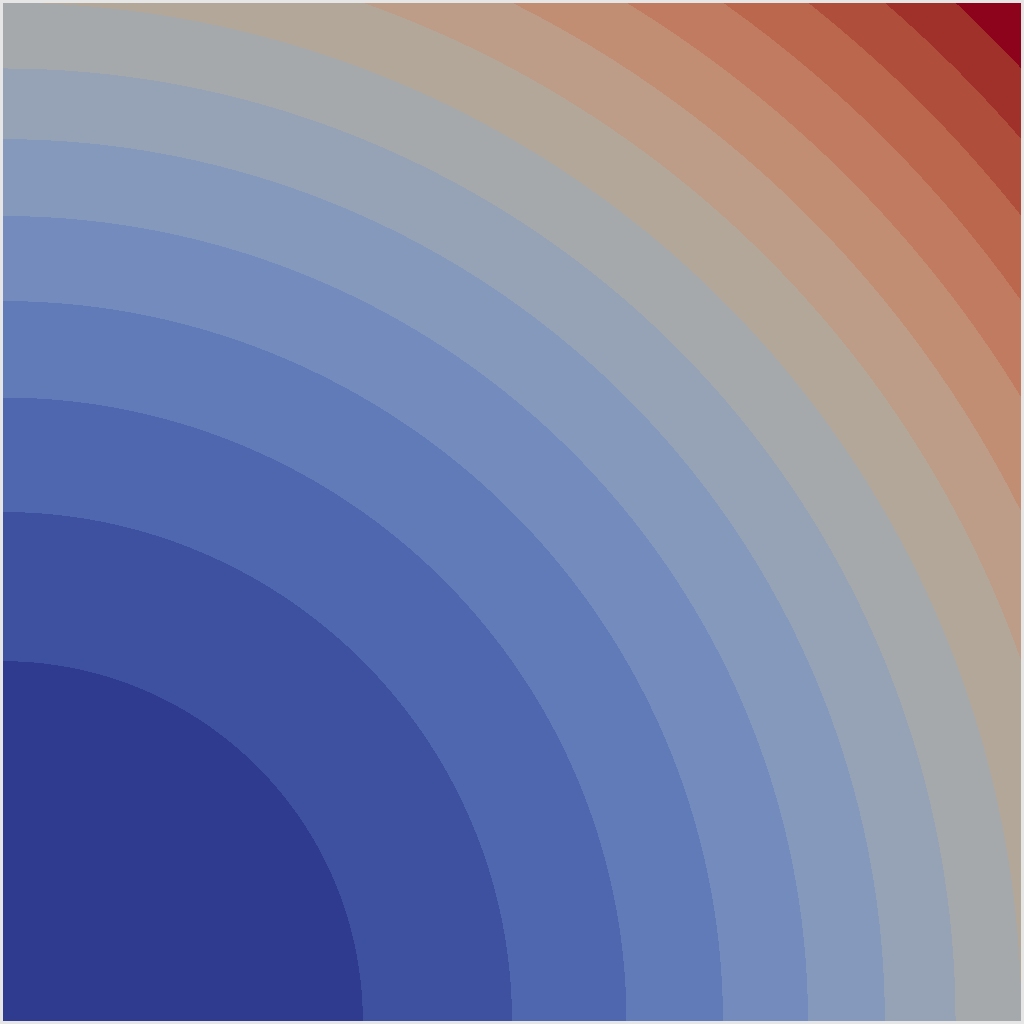
\includegraphics[width=0.32\textwidth]{eta0}\hfill
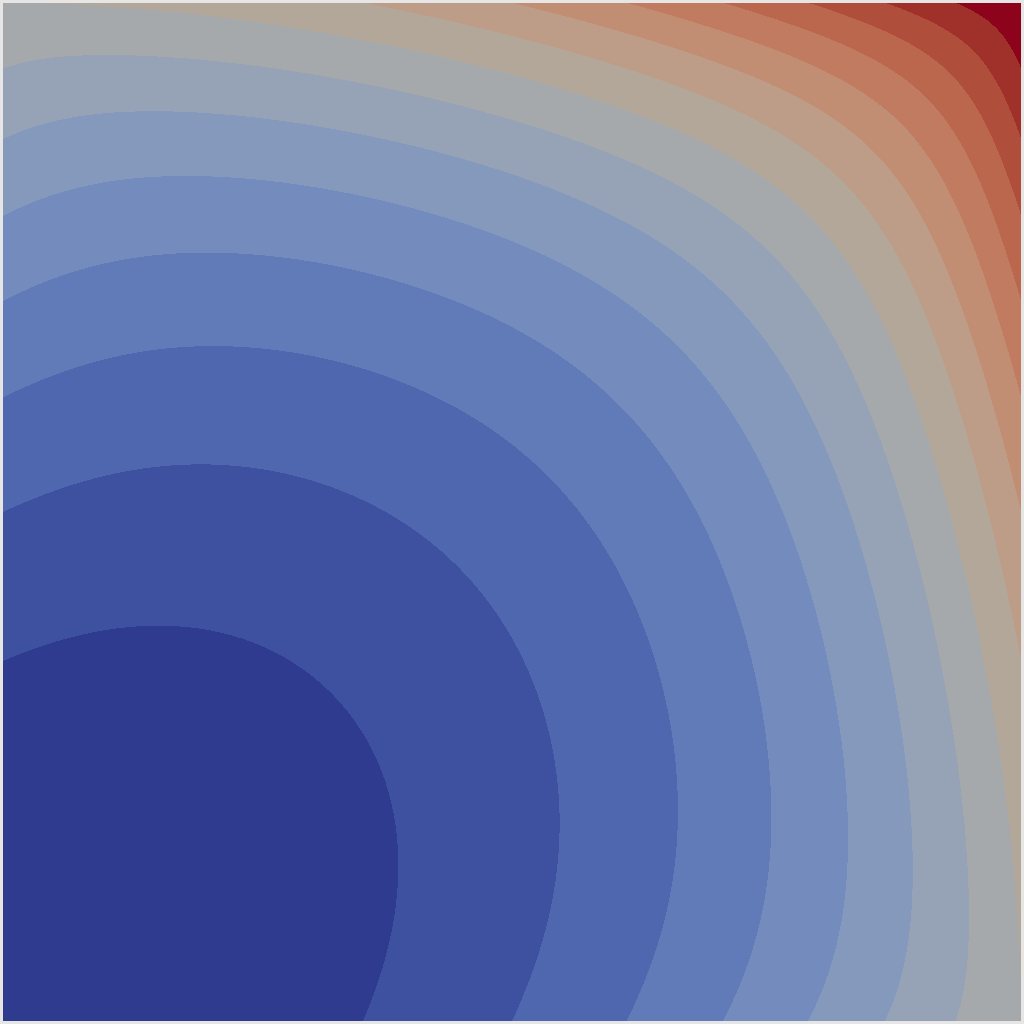
\includegraphics[width=0.32\textwidth]{eta10}\hfill
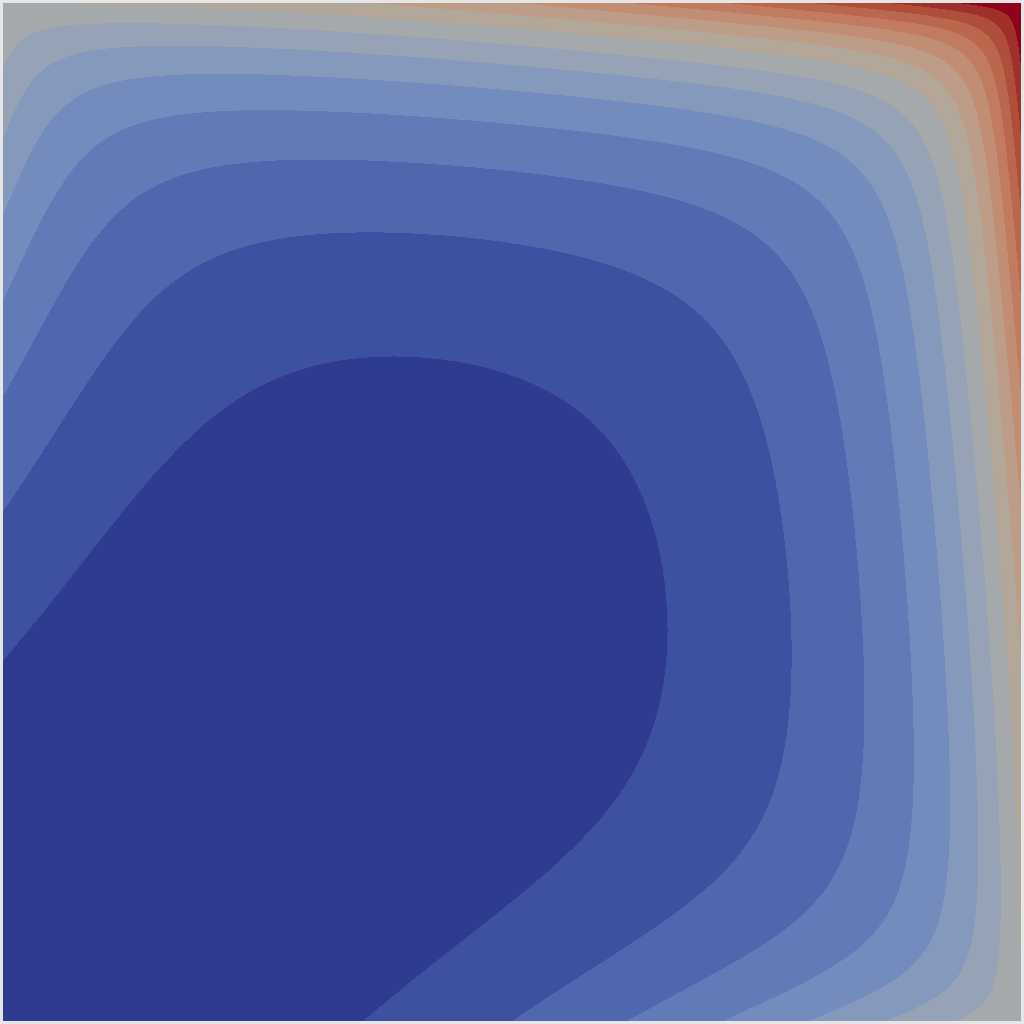
\includegraphics[width=0.32\textwidth]{eta100}
\end{center}
\caption{Illustration of the influence of the parameter $\eta$
in nonlinearity on the solution. $\eta=0$ (left), $\eta=10$ (middle), $\eta=100$ (right).}
\label{fig:1}
\end{figure}

\section{Outlook}

Here are some suggestions how to test and modify this example:
\begin{itemize}
\item Play with other nonlinearities, e.g. $q(u)=\exp(au)$.
\item Compare cost and accuracy of different polynomial degrees and
simplicial meshes vs. cube meshes.
\item Implement Nitsche's method to incorporate Dirichlet boundary conditions 
in a weak sense. This method is based on the following residual form:
\begin{equation*}
\begin{split}
r^{\text{Nitsche}}(u,v) &= \int_\Omega \nabla u \cdot \nabla v + (q(u)-f)v\,dx + \int_{\Gamma_N} jv\,ds \\
&\quad - \int_{\Gamma_D} \nabla u \cdot\nu v\,ds - \int_{\Gamma_D} (u-g)\nabla v \cdot\nu\,ds 
+ \eta \int_{\Gamma_D} (u-g)v\,ds
\end{split}
\end{equation*}
and requires an additional method \lstinline{alpha_boundary} with the following interface:
\begin{lstlisting}[basicstyle=\ttfamily\small,
frame=single,
backgroundcolor=\color{listingbg}]
template<typename IG, typename LFSU, typename X, 
         typename LFSV, typename R>
void alpha_boundary (const IG& ig,
                     const LFSU& lfsu_s, const X& x_s, 
                     const LFSV& lfsv_s, R& r_s) const
\end{lstlisting}

\item Implement the streamline diffusion method for a convection term, see \cite{Elman2005} for details.
\end{itemize}

% bibtex bibliography
\bibliographystyle{plain}
\bibliography{tutorial01.bib}

\end{document}
